% renamed file to z5labpic.tex 2013.02.25 and use standalone class
% zn: 2010.3.11 tikzcreatedpdf.tex
% check out Externalization Library in the pgf-tikz manual v2.0

%--------------------------------------------------------------------------
\documentclass
%{article}
{standalone}
%--------------------------------------------------------------------------
<<<<<<< HEAD
%\usepackage[american]{circuitikz}
\usepackage{tikz}
%	\usetikzlibrary{calc}
=======
\usepackage{tikz}
	\usetikzlibrary{calc}
>>>>>>> a7fba7a3f6cde200aab2b482244b970ba962c31b
	\usetikzlibrary{circuits.ee.IEC}
%	\usetikzlibrary{shapes,decorations,shadows}
%	\usetikzlibrary{decorations.pathmorphing}
%	\usetikzlibrary{decorations.shapes}
%	\usetikzlibrary{decorations.text}
%	\usetikzlibrary{fadings}
%	\usetikzlibrary{fit,chains}
%	\usetikzlibrary{patterns}
	\usetikzlibrary{positioning}
%	\usetikzlibrary{decorations.footprints}
%	\usetikzlibrary{decorations.fractals}
	\usetikzlibrary{scopes}
%	\usetikzlibrary{shapes.gates.logic.IEC}
%	\usetikzlibrary{shapes.gates.logic.US}
%	\usepgflibrary{shapes}
\usepackage{pgfplots}
\usepackage{shortvrb} \MakeShortVerb{\"}
\usepackage{multicol} 
\usepackage{verbatim}
%--------------------------------------------------------------------------
\begin{document}
%--------------------------------------------------------------------------
<<<<<<< HEAD
%----measure internal resistance of battery
% simple solution uses absolute positioning
%\begin{tikzpicture}[circuit ee IEC,
%	set resistor graphic	= var resistor IEC graphic,
%	meter/.style={circle,draw}]
%\draw 
%	(2,0) node[meter](ammeter) {$A$} 		% location of Ammeter
%	(-1,1) node[meter](voltmeter) {$V$}	% location of Voltmeter
%	(0,2) to[battery={info={$\mathcal E$}}](0,0)
%	(0,2) to[make contact] (3.5,2)
%	(0,0) -- (ammeter) -- (3.5,0)
%	(3.5,2) to[resistor={info'=$R$}] (3.5,0)
%	(0,2) -| (voltmeter) |- (0,0);
%	;				
%\end{tikzpicture}

%\begin{tikzpicture}[circuit ee IEC,
%	set resistor graphic	= var resistor IEC graphic,
%	meter/.style={circle,draw}]
%\node at (2,0) (ammeter)[meter] {$A$};
%\node at (-1,1) (voltmeter)[meter] {$V$};
%\node at (0,0) (gnd) {};		% ground potential
%\node at (0,2) (pos) {};		% positive potential
%\draw 
%	(pos) to[battery={info={$\mathcal E$}}](gnd)
%	(pos) to[make contact] (3.5,2)
%	(gnd) -- (ammeter) -- (3.5,0)
%	(3.5,2) to[resistor={info'=$R$}] (3.5,0)
%	(pos) -| (voltmeter) |- (gnd);
%	;				
%\end{tikzpicture}

% solution uses relative positioning. \coordinates provides real points
% \nodes draw lines from their boundaries
% more complicated solution, but hopefully easier to maintain
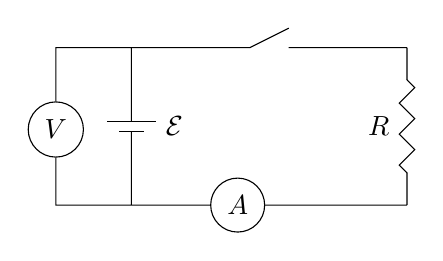
\begin{tikzpicture}[circuit ee IEC,
	set resistor graphic	= var resistor IEC graphic,
	meter/.style={circle,draw}]
\coordinate (gnd);									% ground terminal
\coordinate [above = 2cm of gnd] (pos);		% positive terminal
\coordinate [right = 3.5cm of pos] (top);	% top, far right point of circuit
\coordinate [right = 3.5cm of gnd] (bot);	% bot, far right point of circuit
\node[meter] (ammeter) [right=of gnd] {$A$};
\node[meter] (voltmeter) [above left=1cm of gnd] {$V$};
\draw
	(pos) to[battery={info={$\mathcal E$}}](gnd)
	(pos) to[make contact] (top)
	(top) to[resistor={info'=$R$}] (bot)
	(gnd) -- (ammeter) -- (bot)
	(pos) -| (voltmeter) |- (gnd);
	;				
\end{tikzpicture}

%----batteries in series and parallel
%\begin{tikzpicture}[circuit ee IEC]	% in series
%\draw 
%	(0,2) to[battery={info'={$\mathcal E_1$}}](2,2)
%	to[battery={info'={$\mathcal E_2$}}](3,2)
%	(0,0) to[battery={info'={$\mathcal E_1$}}](2,0)
%	(3,0)to[battery={info={$\mathcal E_2$}}](2,0)	
%	;
%\end{tikzpicture}	
%\qquad
%\begin{tikzpicture}[circuit ee IEC] %  in parallel
%\draw	
%	(0,0) -| (0.5,0.5) -- (1,0.5) to[battery={info=$\mathcal E_1$}]
%	(3,0.5) -- (3.5,0.5) |- (4,0)
%	(0.5,0) |- (1,-0.5) to[battery={info'=$\mathcal E_2$}]
%	(3,-0.5) -| (3.5,0);
%\end{tikzpicture}	
=======
%----batteries in series and parallel
\begin{tikzpicture}[circuit ee IEC]	% in series
\draw 
	(0,2) to[battery={info'={$\mathcal E_1$}}](2,2)
	to[battery={info'={$\mathcal E_2$}}](3,2)
	(0,0) to[battery={info'={$\mathcal E_1$}}](2,0)
	(3,0)to[battery={info={$\mathcal E_2$}}](2,0)	
	;
\end{tikzpicture}	
\qquad
\begin{tikzpicture}[circuit ee IEC] %  in parallel
\draw	
	(0,0) -| (0.5,0.5) -- (1,0.5) to[battery={info=$\mathcal E_1$}]
	(3,0.5) -- (3.5,0.5) |- (4,0)
	(0.5,0) |- (1,-0.5) to[battery={info'=$\mathcal E_2$}]
	(3,-0.5) -| (3.5,0);
\end{tikzpicture}	
>>>>>>> a7fba7a3f6cde200aab2b482244b970ba962c31b

%%----single dry cell measurement
%\begin{tikzpicture}[circuit ee IEC,
%	set resistor graphic	= var resistor IEC graphic,
%	meter/.style={circle,draw}]
%\draw 
%	(0,2) to[battery={info'={$\mathcal E$}}](0,0)
%%	(0,2) -- (3,2)										% top line
%	(0,0) -- (3,0)										% bottom line
%	(3,1) node[meter](voltmeter)	{$V$}	 			% location of V	
%	(0,2) to[make contact] (3,2)
%	(3,2) -- (voltmeter) -- (3,0);
%\end{tikzpicture}

%----schematic for ohm's law measurement
%\begin{tikzpicture}[circuit ee IEC,
%	set resistor graphic	= var resistor IEC graphic,
%	meter/.style={circle,draw}]
%\draw (0,3) to[battery={info'={$\mathcal E$}}](0,0)
%		(0,3) to[make contact] (2,3) 
%%		(3,3) node[meter](ammeter){$A$}(4,3)		% top line 
%		(0,0) -- (4,0);									% bottom line
%\draw
%	(2,2.3) node[meter](ammeter)		{$A$}			% location of A
%	(4,0.9) node[meter](voltmeter)	{$V$}; 		% location of V
%\draw (2,3)--(ammeter) to[resistor={info'={$R$}}] (2,0)	% A,R vertical
%		(2,1.8)-|(voltmeter) -- (4,0);					% V vertical
%\end{tikzpicture}

%\begin{tikzpicture}[circuit ee IEC,
%	set resistor graphic	= var resistor IEC graphic,
%	meter/.style={circle,draw}]
%\draw 
%	(0,2) to[battery={info'={$\mathcal E$}}](0,0)
%	(2.4,2) node[meter](ammeter){$A$}				% location of A
%	(4.5,1) node[meter](voltmeter)	{$V$}	 		% location of V	
%	(0,2) to[make contact] (2,2) -- (ammeter) -- (3.5,2)
%	(3.5,2) to[resistor={info'=$R$}] (3.5,0)
%	(3.5,2) -| (voltmeter) |- (0,0);
%\end{tikzpicture}

%----3 resistors in series
%\begin{tikzpicture}[circuit ee IEC,set resistor graphic=var resistor IEC graphic]
%	\draw (0,0)
%		to[resistor={info'=$R_1$}]			(1.5,0)
%		to[resistor={info'=$R_2$}]			(3.5,0)
%		to[resistor={info'=$R_3$}]			(5,0);
%\end{tikzpicture}
%\hfill
%\begin{tikzpicture}[circuit ee IEC,set resistor graphic=var resistor IEC graphic]
%	\draw (0,0)
%		to[resistor={info'=$R_1$}]			(2,0)
%		to[resistor={info'=$R_2$}]			(4,0)
%		to[resistor={info'=$R_3$}]			(6,0);
%\end{tikzpicture}
%\hfill
% 3 resistors in parallel
%\begin{tikzpicture}[circuit ee IEC,set resistor graphic=var resistor IEC graphic]
%	\draw (0,0) to[resistor={info=$R_1$}]	(0,1.5)
%		(2,1.5 ) to[resistor={info'=$R_2$}]		(2,0)
%		(4,1.5) to[resistor={info'=$R_3$}]		(4,0)
%		(-1,0) -- (4,0)
%		(-1,1.5) -- (4,1.5);
%\end{tikzpicture}

<<<<<<< HEAD
=======

>>>>>>> a7fba7a3f6cde200aab2b482244b970ba962c31b
%--------------------------------------------------------------------------
\end{document}
%--------------------------------------------------------------------------

%----voltmeters
\begin{comment}	% battery + resistor
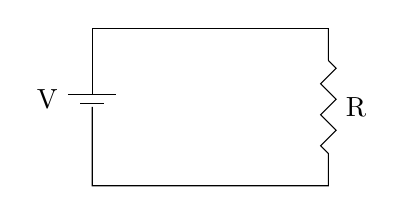
\begin{tikzpicture}[circuit ee IEC,set resistor graphic=var resistor IEC graphic]
	\node (V1) [battery={info'=V},point down] at (0,0.1) {};
%	\draw (0,1) to[make contact={info'=S}]	(2,1)
	\draw (0,1)--(3,1);
	\draw (3,1)	to[resistor={info=R},point down]	(1,3) -- (0,-1) -- (0,0);
	\draw (2,1) -- (3,1); \draw (V1) -- (0,1);
\end{tikzpicture}
\end{comment}
